\section{Diagrama de la Estructura General del Sistema} 
La Figura \ref{fig:Diagrama de sistemas} ilustra la arquitectura general del proyecto propuesto, mostrando por separado cada uno de los diferentes sistemas que conforman este proyecto y el servicio en el que están alojados algunos de los sistemas. 
El presente diagrama muestra un sistema basado en microservicios, en el que se separa la lógica de la red neuronal de la parte del servidor. Por otro lado, dentro del servidor Java, apesar de tener toda la lógica dentro del mismo, existe la posibilidad de separar la lógica de la simulación del SAES, de la lógica del sistema móvil.

Como punto de partida está la base de datos, la cual está alojada en Railway. Esta abse de datos es la encargada de guardar todos los datos tanto de alumnos, docentes y el personal de seguridad, así como de otros datos académicos. Cabe recalcar que esta base de datos es una simulación de la base de datos de la página original del SAES, la cual se plantea compartir con el presente sistema móvil.

Posterior a esto, se tiene al servidor Java, el cual se encarga de procesar todas las solicitudes que haga el usuario dentro de la app móvil o del simulador del SAES. Esta parte del sistema se encuentra alojada en Azure. Este servidor se comunica tanto con el sistema web de la simulación del SAES, como con la app móvil, a través de solicitudes HTTPS.

A su vez, se encuentra el servidor de la red neuronal, alojado igualmente en Azure. Este servidor, como su nombre lo indica, se encarga únicamente de procesar todas las solicitudes para realizar el reconocimiento facial de los estudiantes dentro de la aplicación móvil. Sin embargo, para poder obtener los vectores de características de cada alumno y que se pueda hacer el reconocimiento facial de manera adecuada desde la app, se tiene la comunicación del sistema web con este mismo servidor. El sistema web cuenta con un módulo de registro de alumnos, en el cual se le toma un video de 5 segundos, para obtener diferentes fotos desde diferentes ángulos, y así, guardar el vector de características del alumno en el momento en el que se realizó su registro. De esta forma, al realizar el reconocimiento facial desde la aplicación móvil, tendrá un punto de partida para comparar con la foto que se le tome desde la aplicación móvil.

\begin{figure}[htbp!]
	\begin{center}
		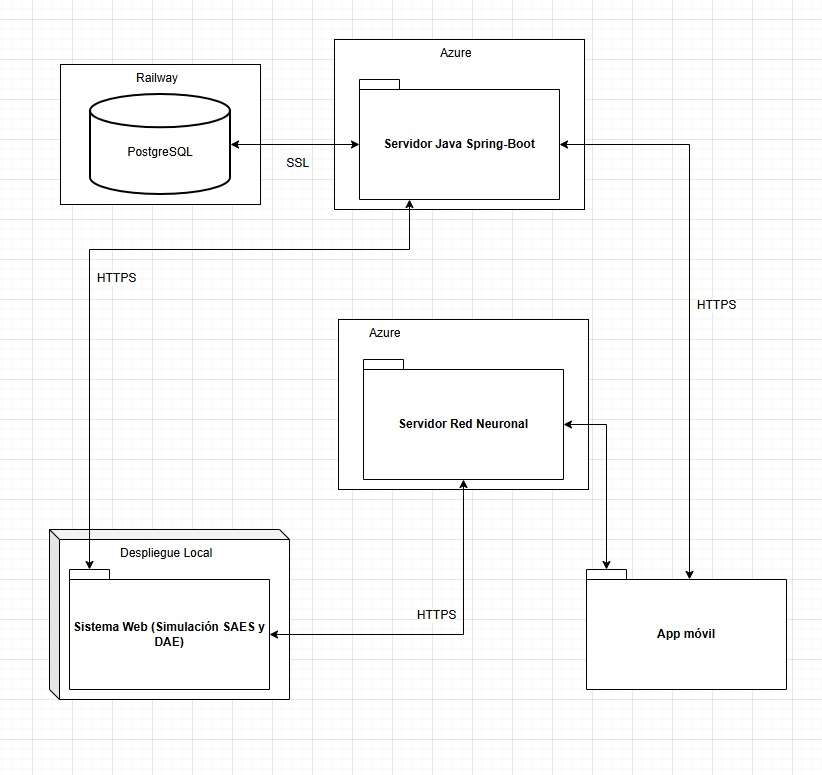
\includegraphics[width=0.9\textwidth]{images/DiagramaGeneralClases}
		\caption{Diagrama de la Estructura General del Sistema.}
		\label{fig:Diagrama de sistemas}
	\end{center}
\end{figure}

A continuación se entrara más en detalle en la estructura interna de los componentes del sistema del diagrama anterior.
